%\chapter{Hinweise}
%
%Ist die Architektur richtig gewählt?! Node.js für Asynchrone Webaufrufe deutlich besser! Als Anmerkung ins Fazit packen und Auswahl von PHP auf vorhandenes Wissen  schieben!\\
%
%Ausblick: Technik muss besser werden, Schwachstellen in Usability\\
%
%Acronym \acf{CAS}\\
%
%Internet-Source in footnote\footnote{\citep{cas}}\\
%
%Book-Source in footnote\footnote{\citep{einfuehung_sap_hana}}\\
%
%\begin{figure}[H]
%	\centering
%	{
\includegraphics[height=5cm]{Bilder/logo_dhbw_ma.jpg}}
%	\caption{Example of a figure \protect\citep[page 32]{cas}}
%	\label{fig:Example}
%\end{figure}

\chapter{Reflexion}
Das folgende Kapitel beschäftigt sich mit der kritischen Reflexion der Leistung und Entscheidungen des Projektteams und bezieht sich ausschließlich auf die Software.\\

\begin{figure}[H]
	\centering
	{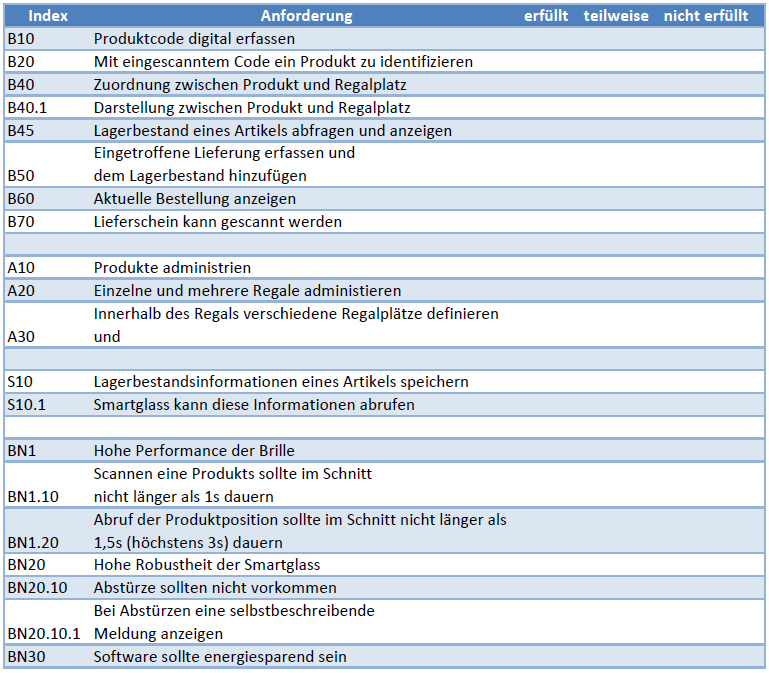
\includegraphics[scale=0.73]{Bilder/Abbildungen/anforderungen_zusammenfassung_bewertung.png}}
	\caption{Übersicht der Anforderungen mit Erfüllungsgrad}
	\label{fig:anforderungen_erfuellt}
\end{figure}

Während die grundlegende Architektur, das Projekt \ac{SMAR} in einer Thin Client-Server-Architektur aufzubauen, in diesem Szenario durchaus Sinn macht, da in der Anwendung mehrere Clients vorhanden sind, die alle auf dieselben Daten - teilweise gleichzeitig - zugreifen, würde eine Berechnung der Daten auf den Clients inkonsistente Stände verursachen und die Performanz negativ beeinflussen. Außerdem waren die eingesetzten Technologien auf den Smartglasses durch das Android Betriebssystem weitestgehend vorgegeben. Entscheidungen wie \zB das Benutzen der ZBar Library, statt der ZXing Anwendung zur Bar-Code-Erkennung sorgen dafür, dass das Projekt eigenständig funktioniert und keine weiteren Softwarevoraussetzungen benötigt. Die \ac{REST} \ac{API} erzeugt eine einfache Kommunikation zwischen Clients (Web Administration und Android-App) und Server und wird von allen Teilen sehr gut unterstützt. Die Web Administration jedoch, die größtenteils eine asynchrone Kommunikation benutzt, kommuniziert im Hintergrund mit PHP-Skripten. Dies ist vor Allem aufgrund der asynchronen Arbeitsweise sehr kompliziert gelöst und nicht zeitgemäß. Hier wäre es von Vorteil gewesen einen NodeJS-Server mit einem AngularJS-Webfrontend einzusetzen. Dies hätte die Programmierung vereinfacht und deutlich Zeit gespart.\\

Das zu Beginn der Entwicklung vereinbarte Zeitmanagement wurde durch das gesamte Projektteam nicht eingehalten. Betrachtet man entsprechende Pushs auf dem Git-Repository sind deutliche Fortschritte zu Anfang des Projekts, zu Anfang des Jahres und zu Ende des Projekts zu verzeichnen. Eine bessere Verteilung und ein kontinuierlicheres Arbeiten am Projekt hätten das Ergebnis verbessern und Schwachstellen in der Architektur und Technologieauswahl frühzeitig aufdecken können.

\chapter{Ausblick}
\label{cha:ausblick}
Im gesamten Projektverlauf wurde sowohl in der Hard- als auch in der Software erkannt, dass sich das Shelf Management mit Wearable Computern noch in einem frühen Stadium befindet. Dennoch kann das Potential hinter dieser Technologie in Verbindung mit dieser Software erkannt werden. Eine Wiederaufnahme des Projekts könnte fehlende oder wünschenswerte Funktionen hinzufügen, die im folgenden als Möglichkeiten erläutert werden sollen.\\

\ac{SMAR} beschäftigt sich, wie der Titel bereits sagt, vor allem auch mit Augmented Reality. Dies wurde im Rahmen dieses Projektes mit Vektorgrafiken dargestellt, die die Realität nachbilden und dem Benutzer eine Orientierung in der realen Welt vermitteln sollen. Durch entsprechende Analysen von Vorschaubildern der integrierten Kamera könnte auf die Darstellung der Regale über Grafiken verzichtet werden. Stattdessen wäre eine Manipulation der Kamerabilder denkbar, in denen die ausgewählte Section eines Regales im Sichtfeld markiert wird. Dies würde dem Benutzer das Übertragen der fiktiven Welt auf die reale Welt ersparen und er könnte sich noch effektiver auf die eigentliche Aufgabe konzentrieren.\\
Die eingebaute Kamera, sowie hauptsächlich das Display müssten jedoch eine deutlich höhere Qualität für ein zufriedenstellendes Ergebnis liefern.\\
Bei Geräten, die eine entsprechende Kamera nicht besitzen oder von der Handhabung nicht für Augmented Reality geeignet sind (wie \zB Smartphones), würden bereits von einer Erweiterung der SVG-Grafiken um Produktbilder am korrekten Regalplatz profitieren. Der Benutzer würde zwar noch nicht das reale Regal sehen, könnte die SVG-Grafiken anhand der realen Produktbilder aber leichter mit der Realität verknüpfen.\\

Im Rahmen dieser Arbeit wurde ausschließlich das Finden der Section innerhalb eines Regales betrachtet. Dies ist für kleinere Einzelhandelsfilialen durchaus ausreichend. Eine Nummerierung der Regale reicht aus, um dem Mitarbeiter die nötigen Informationen für eine effiziente Suche zu geben. Betrachtet man den Großhandel mit großen Lagerhallen und mehreren hunderten Regalen, so wird eine reine Nummerierung nicht mehr reichen, um dem Mitarbeiter das richtige Regal anzuzeigen. Der Mitarbeiter benötigt eine Navigationshilfe. Mit Hilfe von Triangulationsverfahren wäre es möglich eine Indoor-Navigation in \ac{SMAR} zu integrieren. Der Mitarbeiter bekäme so nicht nur den Regalplatz mitgeteilt, sondern eine genaue Navigation auf Grundlage seines Standorts.\\
Im Zuge der Positions- und Wegeoptimierung kann man daraus noch weitere Optimierungen treffen. Es ist dann denkbar, dass der Mitarbeiter quasi nicht mehr einzelne Artikel einscannen muss, und die Smartglass dann den Weg bzw. das Bild des Regals anzeigt, sondern, dass der Mitarbeiter einen Code scannt, zum Beispiel einen Code an einer Palette, der alle Artikel enthält. Die Smartglass berechnet dann anhand der Artikel und der genauen Position in der Filiale den optimalen Weg, den der Mitarbeiter laufen muss, um am einfachsten und effizientesten die Ware einzuräumen. Zusätzlich wird das Scannen der einzelnen Produkte überflüssig und erhöht so noch einmal die Effizienz.\\

Im vorgegebenen Zeitrahmen war es darüber hinaus nicht mehr möglich das Android Notification Center in die App einzubinden. Die technischen Voraussetzungen sind gegeben, sodass ein Implementieren der folgenden Funktionalität ohne weitere Librarys möglich wäre. Das Projekt \ac{SMAR} beschäftigt sich mit der Warenannahme und der Wareneinräumung. Dadurch müssen die Lager- und Regalbestände dem Projekt jederzeit bekannt sein. Diese Daten könnte man nutzen, in dem der Benutzer in der App (\zB über das Android Notification Center) benachrichtigt wird, sobald der Regalbestand eine untere Grenze unterschreitet \bzw eine E-Mail an den zuständigen Mitarbeiter versendet wird, sobald der Lagerbestand eine definierte untere Grenze unterschreitet. Unzufriedene Kunden aufgrund von fehlenden Beständen könnten damit zuverlässig verhindert werden. Neben den technischen Voraussetzungen sind die Vorbereitungen in der Datenbank und der Web Administration - durch die Definition der unteren Grenze - bereits getroffen. Für den E-Mail-Versand müsste der Anwendung jedoch ein Service, \zB in Form eines Cron-Jobs hinzugefügt werden, welcher die Lagerbestände regelmäßig prüft.\\

Ein weiterer, für die Usability der App entscheidender Faktor ist die Eingabemethode. Aktuell (Stand: Mai 2015) werden die vier Hardwareknöpfe zur Navigation durch das Android Betriebssystem und der \ac{SMAR}-App benutzt. Dies ist oft sehr umständlich und benötigt eine freie Hand. Als Alternative wurde die Spracherkennung bereits in Kapitel \ref{cha:technik} \nameref{cha:technik} genannt, die aufgrund von mangelnder Qualität - vor allem in lauten Umgebungen - allerdings nicht praktikabel war. Zukünftige Versionen von Smartglasses können eine verbesserte Spracherkennung mit Unterstützung der deutschen Sprache beinhalten. Eine Implementation der Spracherkennung in die App könnte die Eingabe erheblich erleichtern und die Effizienz bei Erledigung der Aufgaben nochmals erhöhen.\\
Um darüber hinaus die Augen des Benutzers zu entlasten, wäre außerdem die Nutzung der Android \glqq android.speech.tts.TextToSpeech\grqq -Klasse denkbar. Diese Klasse ermöglicht die Sprachausgabe von eingegebenem Text. Zusatzinformationen, wie \zB der Lagerbestand, könnten durch die Lautsprecher der Smartglasses an den Benutzer übergeben werden. Ein angenehmerer Tragekomfort wäre die Folge, da die Augen durch das kleine und qualitativ niederwertige Display angestrengt werden.\\

Ein weiterer, neuer Aspekt, der in dieser Arbeit noch nicht behandelt wurde, ist der Umgang mit Reklamationen. Es ist durchaus denkbar, wenn man Ware vom Lieferanten erfasst und dem Bestand hinzufügt, dass Reklamationen ähnlich behandelt werden. Dabei muss natürlich unterschieden werden, ob die Ware defekt oder wiederverkaufbar ist. Somit hätte man einen sehr aktuellen Lagerbestand und gleichzeitig auch eine Liste aller Reklamationen. Dies würde nachträgliches und vor Allem manuelles Erfassen überflüssig machen, wodurch wieder Zeit gespart werden kann. \\

Eine andere Form der Reklamation ist jene seitens der Filiale, wenn sie Ware vom Lieferanten aufgrund von Qualitätsgründen oder falscher Lieferung ablehnt. Auch dies muss erfasst und kategorisiert werden. Im Zuge der Einführung von Wearable Computern können Routinen geschaffen werden, sodass nach dem Scann der Bestellung diese abgelehnt werden. Auch dadurch spart man nachträgliche Erfassungen und somit Zeit und hat gleichzeitig aktuelle Informationen im System. \\

Rückblickend auf diesen Abschnitt sieht man, dass es noch sehr viele, weitere und auch komplexere Anwendungsgebiete einer Smartglass oder allgemeiner von Wearable Computern im Bereich des Einzelhandels gibt. 
%Das folgende Kapitel beschreibt den möglichen Ausblick einer Shelf Management Software in Verbindung mit einer Augmented Reality Smartglass aus Sicht der Projektteilnehmer. \\
%
%Der angezeigte Ausschnitt eines Regals ist bei dieser Software nur sehr schematisch gewesen. Außerdem wurde bereits im vorherigen Verlauf der Arbeit darauf verwiesen, dass es durchaus denkbar ist, und die Architektur darauf ausgelegt ist, die Kamera der Smartglass dauerhaft mitlaufen zu lassen. Mit zusätzlicher Positionsbestimmung in der Filiale und dauerhafter Kommunikation mit dem Server im Backoff ist bestimmt eine noch bessere und genauere Zielführung zu einem Regalplatz möglich. 
%\\
%Aufgrund der schwachen Auflösung der Kamera, ist es erforderlich die entsprechenden Codes sehr nah an die Linse zu halten, was in einem Live-Betrieb die Arbeit eher behindert als bereichert. Mit einer höheren Auflösung ist auch ein erfassen von entfernten Codes denkbar, sodass neben der Position des Mitarbeiter auch die Blickrichtung dessen erfasst werden kann. Dies ist quasi eine weitere Dimension, die zur Berechnung hinzugezogen werden kann und genauere Hilfen ermöglicht. 
%\\
%Durch höhere Auflösungen könnten der Mitarbeiter beim Vorbeigehen Produkte einscannen. Dabei könnte ihm angezeigt werden, dass manche Produkte nicht an diesen Regalplatz gehören, weil sie vom Kunden verlegt wurden, und weggeräumt werden müssen. 
%\\
%Vor allem bei frische Produkten ist es vorstellbar in den Barcode ein entsprechendes Mindesthalbarkeitsdatum einzuprägen. Beim Vorbeigehen könnte dieses eingescannt und angezeigt werden. Bei kritischen Fällen oder sogar Überläufen könnte dieses entsprechend markiert werden, sodass es einfach aus dem Verkauf genommen werden könnte.
%\\
%Außerdem ist es wahrscheinlich ratsam zum Scannen einiger Produkte nicht nur die Smartglass zu verwenden, sondern auch andere externe Komponenten, wie einen Ringscanner oder einen üblichen Handscanner, der über Bluetooth mit der Smartglass kommuniziert. So sind einige Prozesse bzw. Bewegungen natürlicher sowie ergonomischer für den Mitarbeiter. 
%\\
%Weiter in die Zukunft gedacht, ist es vorstellbar, dass nicht nur Mitarbeiter eine Smartglass verwenden, sondern die Kunden selbst. dazu wären natürlich hohe Stückzahlen und ein entsprechend verlässliches sowie benutzerfreundliches System notwendig. Allerdings wäre der Kunde vollkommen autark und könnte ohne jegliche Interaktion mit einem Mitarbeiter seine Einkäufe erledigen. Außerdem ist es denkbar, wenn der Kunde eine Smartglass verwendet, dass diesem mehr Produktinformationen, wie Nährstoffe passend zu seiner Diät, oder weitere dazu passende Produkte, ähnlich wie "Kunden kauften auch diesen Artikel", angezeigt werden könnten. 
%\\

\chapter{Fazit}
Die in den ersten Kapiteln beschriebene durchgeführte Analyse stellt den IST-Zustand in gängigen Einzelhandelsfilialen dar und erkennt Bedarf in der Unterstützung der Warenannahme und -einräumung durch Wearable Computer. Der Vergleich verschiedener Gerätetypen unterstreicht die Entscheidung, diese Unterstützung mit Hilfe von Smartglasses umzusetzen. Eine entsprechende Anforderungsanalyse inklusive Priorisierung der zu erledigenden Aufgaben stellen sicher, dass \ac{SMAR} bereits in diesem Umfang der großen Studienarbeit zu einem Mehrwert in Filialen führen und die Effizienz und Effektivität im Unternehmen steigern können.\\

Zu Beachten ist, dass sowohl die Hardware in Form von Smartglasses, als auch die Software noch in einem frühen Stadium stehen und daher nicht alle Funktionen ausgereift sind und optimal funktionieren. Dies wird \zB durch das Display der Vuzix M100 deutlich, welches oft nicht optimal ausgerichtet ist und kleine Texte nicht deutlich genug auflöst.\\

Erschwert wurde die Entwicklung außerdem durch fehlende Testmöglichkeiten in entsprechenden Einzelhandelsfilialen. Die durchgeführte Umfrage bei Managern von solchen Filialen half bei der Bedarfs- und Anforderungsanalyse, allerdings konnte nicht getestet werden, ob diese korrekt verstanden, umgesetzt wurden und ob dies den Wünschen der Mitarbeiter an eine entsprechende Technologie entspricht.\\

Dennoch wurden die aus den Umfragen interpretierten Anforderungen mit erster Priorität umgesetzt und bieten daher - zumindest theoretisch - eine erfolgreiche Grundlage. Darüber hinaus muss beachtet werden, dass die Umsetzung entsprechender Systeme noch nicht existiert und dies einen ersten Entwurf einer Entwicklung darstellt.\\

\ac{SMAR} ist daher nicht als eine fertige und einsetzbare Software in Unternehmen anzusehen. \ac{SMAR} bietet viel mehr die Grundlage für entsprechende Proof-Of-Concepts gegenüber möglichen Kunden und ist für Demonstrationen sehr gut geeignet. Die weitere Entwicklung der Software erfordert eine Zusammenarbeit mit dem Kunden inklusive entsprechender Testphasen.\\

Wird das Projekt entsprechend dem oben beschriebenen Absatz verstanden, ist es als Erfolg anzusehen.